\begin{center}
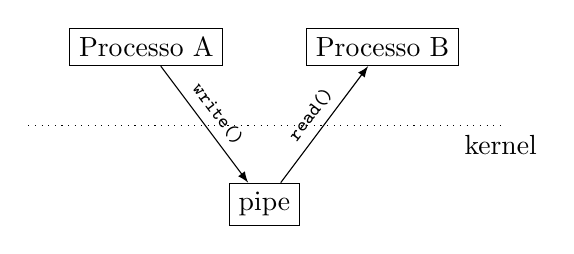
\begin{tikzpicture}
\def\shift{3cm}
\def\yshift{\shift/3}
\tikzset{base/.style={draw},pipe/.style={base},proc/.style={base},
every path/.style={>=latex,draw},syscal/.style={font=\scriptsize\tt}}
\node[pipe] at (\shift,-\yshift) (PIPE) {pipe};
\draw[dotted] (0,0) -- (2*\shift,0) node[below] {kernel};
\node[proc] at (\shift/2,\yshift) (PA) {Processo A};
\node[proc] at (1.5*\shift,\yshift) (PB) {Processo B};
\path[->] (PA) -- node[syscal,rotate=-53,above]{write()} (PIPE);
\path[->] (PIPE) -- node[syscal,rotate=53,above]{read()} (PB);
\end{tikzpicture}
\end{center}
